\documentclass{beamer}
%\documentclass[handout]{beamer}

\usepackage{pgfpages} 
%\pgfpagesuselayout{4 on 1}[letterpaper,border shrink=5mm,landscape] 
%\pgfpagesuselayout{2 on 1}[letterpaper,border shrink=2mm]

\usetheme{default}

\mode<presentation> {
%  \usetheme{Warsaw}
  \usetheme{Frankfurt}
%  \usetheme{Boadilla}
%  \usetheme{Marburg}
}

\mode<handout>{\setbeamercolor{background canvas}{bg=black!5} %
    \pgfpagesuselayout{2 on 1}[letterpaper,border shrink=4mm] }

\title[CAC Intro] {A Brief Introduction to\\ The Center for Advanced Computing}

\begin{document}
  \setbeamercovered{transparent}  
  \begin{frame}
    \titlepage
  \end{frame}

%table of contents
  \begin{frame}{Outline}
    \tableofcontents
  \end{frame}
  
    \note[item]{blah math}
  \section{Resources}
  \subsection {Hardware}
  \begin{frame}{Hardware}
   \begin{block}{Hardware}
    \begin{itemize}
    \item 468 Opteron nodes, over 1282 cores
    \item 1 SGI Altix, 32 cores 96GB Ram
    \item Gigabit networking, Infiniband networking, NUMALink
    \end{itemize}
   \end{block}
  \end{frame}
  \begin{frame}{Hardware: nyx}
   \begin{block}{Nyx}
    \begin{itemize}
    \item nyx is the Opteron cluster
    \item \texttt{nyx-login.engin.umich.edu} is
      the login host for this cluster
    \item Currently has 6TB NFS file system
    \item Running RedHat Enterprise Linux 4
    \end{itemize}
   \end{block}
  \end{frame}
  \begin{frame}{Hardware: bighouse}
   \begin{columns}[c]
    \begin{column}{7cm}
    \begin{block}{Bighouse}
    \begin{itemize}
      \item bighouse is our Itanium SMP machine;
      \item Login: \texttt{bighouse.engin.umich.edu}
      \item Shares nyx's 6TB NFS file system
      \item Running SUsE Linux Enterprise Server 10
      \item ProPack 5 from SGI
    \end{itemize}
   \end{block}
   \end{column}
   \begin{column}{5cm}
    \begin{center}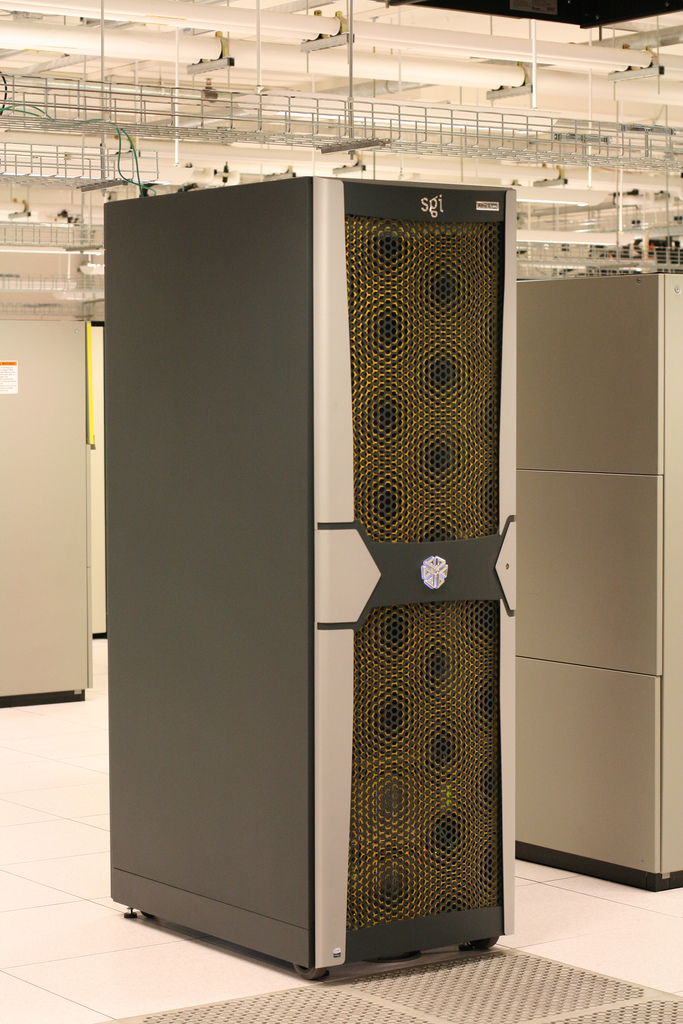
\includegraphics[height=2.7in]{tallbighouse}\end{center}
   \end{column}
   \end{columns}
  \end{frame}
  
  \subsection {Software}
  \begin{frame}{Software}
    \begin{itemize}
    \item openmpi -- MPI libraries
    \item mcnp5 -- Monte Carlo N-Particle Transport
    \item matlab -- matrix math application
    \item fftw -- Fast Fourier Transform Library (parallel and serial)
    \item fluent -- fluid dynamics application
    \item gaussian -- electro-chemical analysis application
    \item java -- Sun's Java Language
    \item mathematica -- symbolic math application
    \item nag -- Numerical Algorithm Group's Fortran Compilers
%    \item netcdf -- data format library
    \item pgi -- Portland Group Compilers
    \item R -- matrix math application
    \item simpson -- solid-state NMR simulation software
    \item and more...
    \end{itemize}
  \end{frame}
\begin{frame}[fragile]
    \frametitle{Current List of Software}
    To get a current list of software on the cluster you are using, type
    \texttt{module~avail}, you'll see something like:
    \tiny
\begin{verbatim}
--------------------- /home/software/rhel4/Modules/3.2.1/modulefiles ---------------------
R/2.2.1-gcc       gaussian/03-64bit mcnp5/1.4         null              radmind/1.5.1  
dot               hdf5/1.6.5-gcc    module-info       openmpi/1.0.1-gcc simpson/1.1.1-gcc  
fftw/2.1.5-gcc    hdf5/1.6.5-pgi    modules           openmpi/1.0.2-gcc simpson/1.1.1-pgi 
fftw/2.1.5-pgi    java/1.5.0_06     nag/7             openmpi/1.0.2-pgi torque 
fluent/6.2        mathematica/5.2   netcdf/3.6.1-gcc  pdsh              use.own 
gaussian/03-32bit matlab/7.1        netcdf/3.6.1-pgi  pgi/6.1(default) 
\end{verbatim}
    \normalsize
    \begin{itemize}
    \item To select a software package, type: \texttt{module~load~\textit{package/version}}.
    \item To see what you have loaded, type: \texttt{module~list}
    \item For help with the \texttt{module} command type: \texttt{module~help}
    \end{itemize}
    We load some basic utilities be default, so when you first log in you will see
    the Torque/PBS commands and the PGI compilers in your list of loaded modules.
\end{frame}
  
  \section{Mechanics: Access}
  \subsection{Transferring files and data to and from the clusters}
  \begin{frame}{Transferring Files}
   \begin{block}{SFTP}
    \begin{itemize}
    \item Files are transferred to the file space on the clusters using either
      Secure Copy (\texttt{scp}) or Secure FTP (\texttt{sftp}).
    \item Your password for file transfers and logins is your UM Kerberos (Level-1)
      password and your login is your Uniqname.
    \end{itemize}
   \end{block}
  \end{frame}
  \begin{frame}{File Transfers: Windows}
    \begin{itemize}
    \item SSH Secure Communications' Secure File Transfer
    \item click ``Quick Connect'': \\
      \begin{center}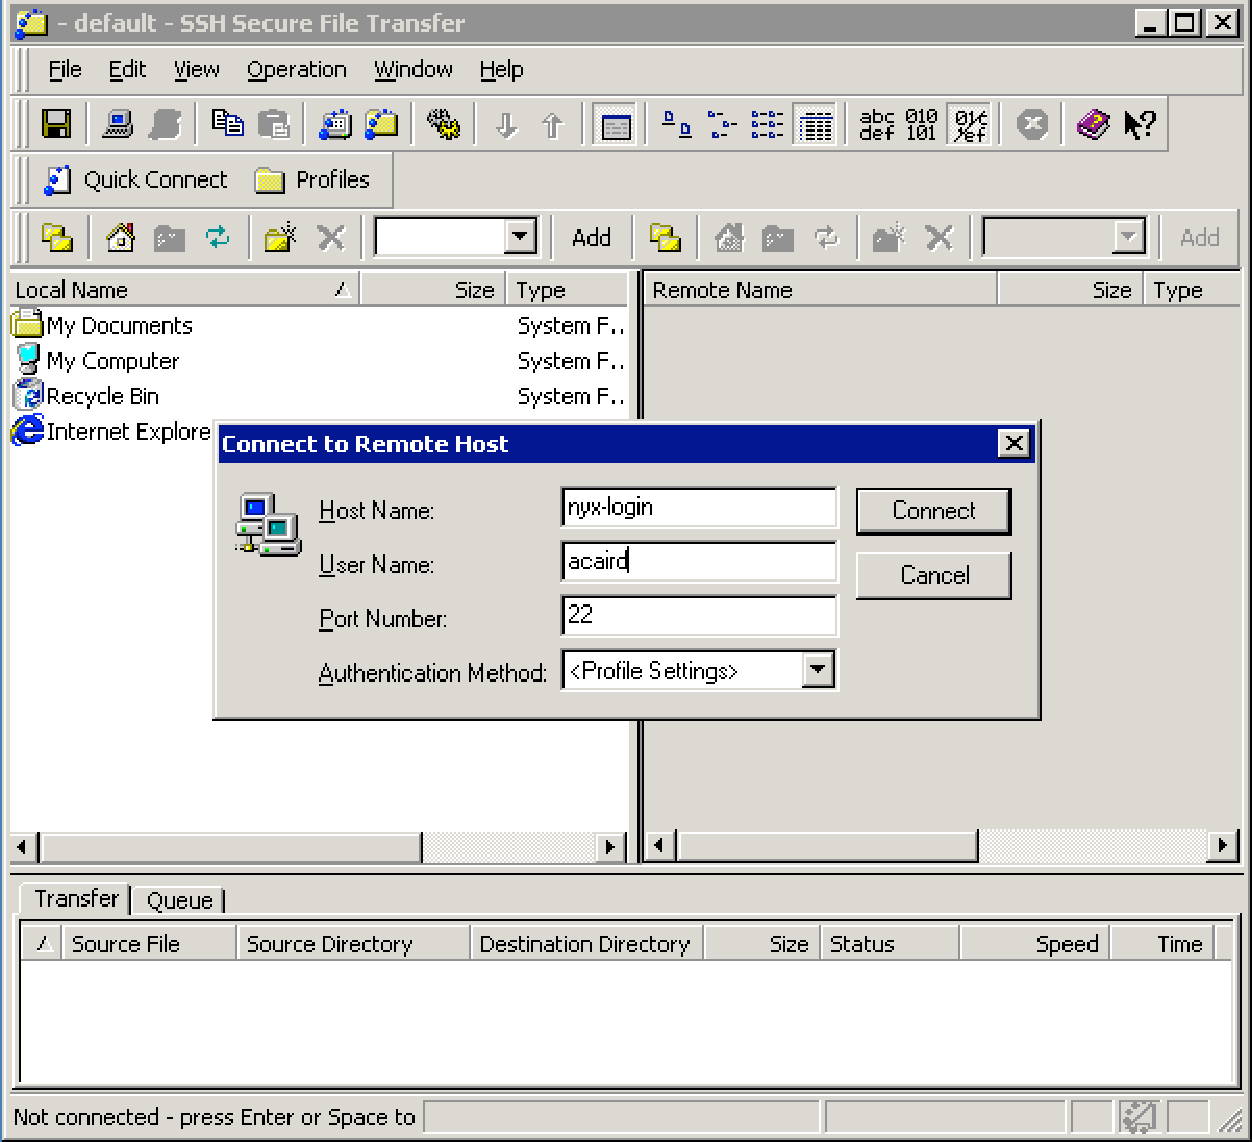
\includegraphics[width=2.5in]{ssh-sftp-login}\end{center}
    \end{itemize}
  \end{frame}
  \begin{frame}{File Transfers: Windows}
    \begin{itemize}
    \item agree to add key to local database (only happens once), click
      ``OK'' on ``SSH Authentication Response''
    \item You will see: \\
      \begin{center}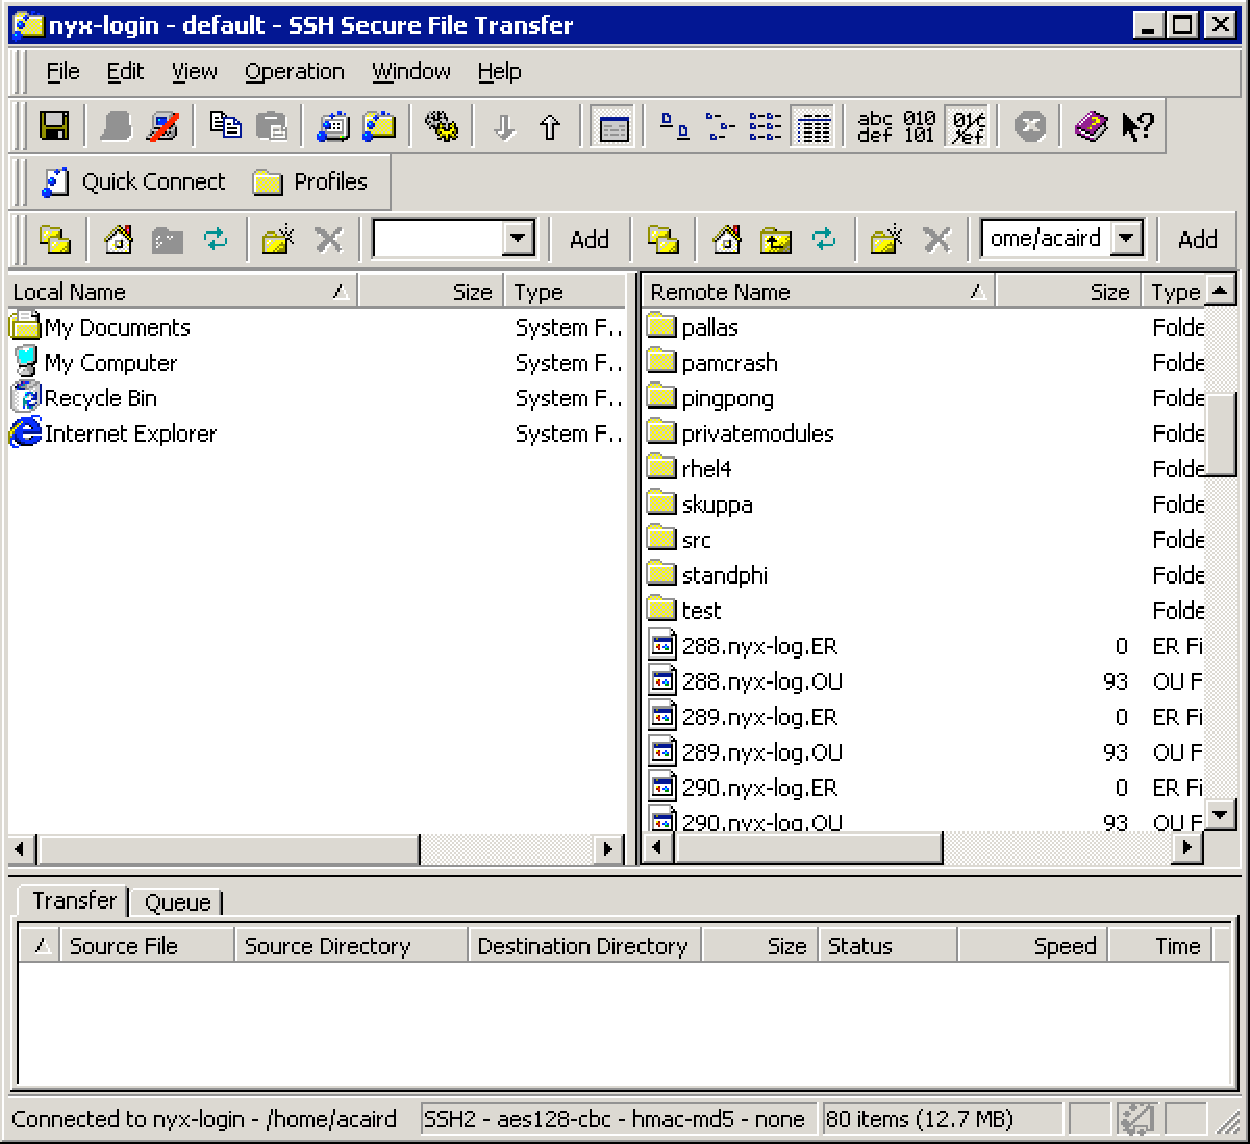
\includegraphics[width=2.48in]{ssh-sftp-connected}\end{center}
    \item You can drag and drop files back and forth
    \end{itemize}
  \end{frame}
  \begin{frame}{File Transfers: Windows}
    \begin{itemize}
    \item There are other programs for Windows besides SSH's SCP
      program, any modern SCP/SFTP program will work
    \item SSH Secure Communications: \url{http://www.ssh.com}
    \item WinSCP: \url{http://winscp.net/eng/index.php}
    \item Putty: \url{http://www.chiark.greenend.org.uk/~sgtatham/putty/}
    \item Cygwin: \url{http://www.cygwin.com/}
    \item lots of others, see Google
    \end{itemize}
  \end{frame}
  \begin{frame}{File Transfers: Mac}
    \begin{itemize}
    \item UM/RSG's Fugu
    \item Fill the in information as shown: \\
      \begin{center}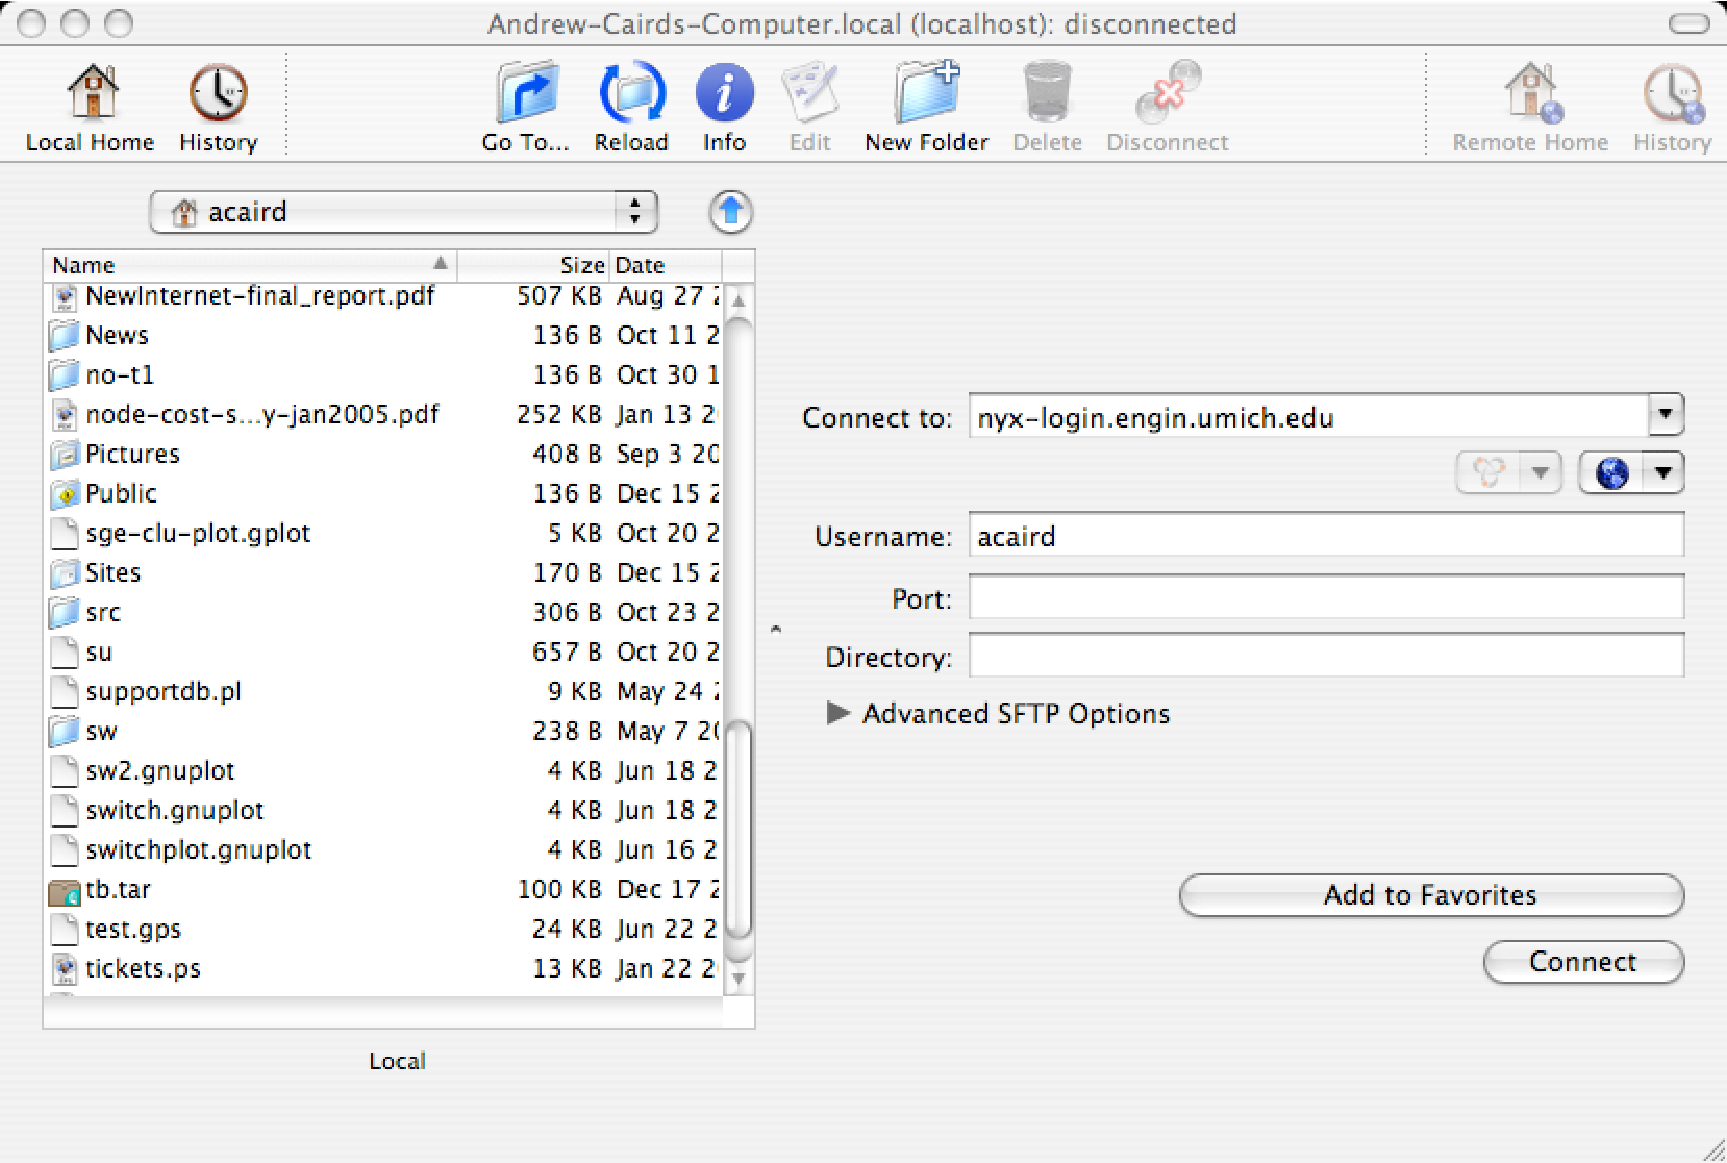
\includegraphics[width=2.5in]{ssh-fugu-login}\end{center}
    \end{itemize}
  \end{frame}
  \begin{frame}{File Transfers: Mac}
    \begin{itemize}
    \item Enter password when prompted
    \item You will see: \\
      \begin{center}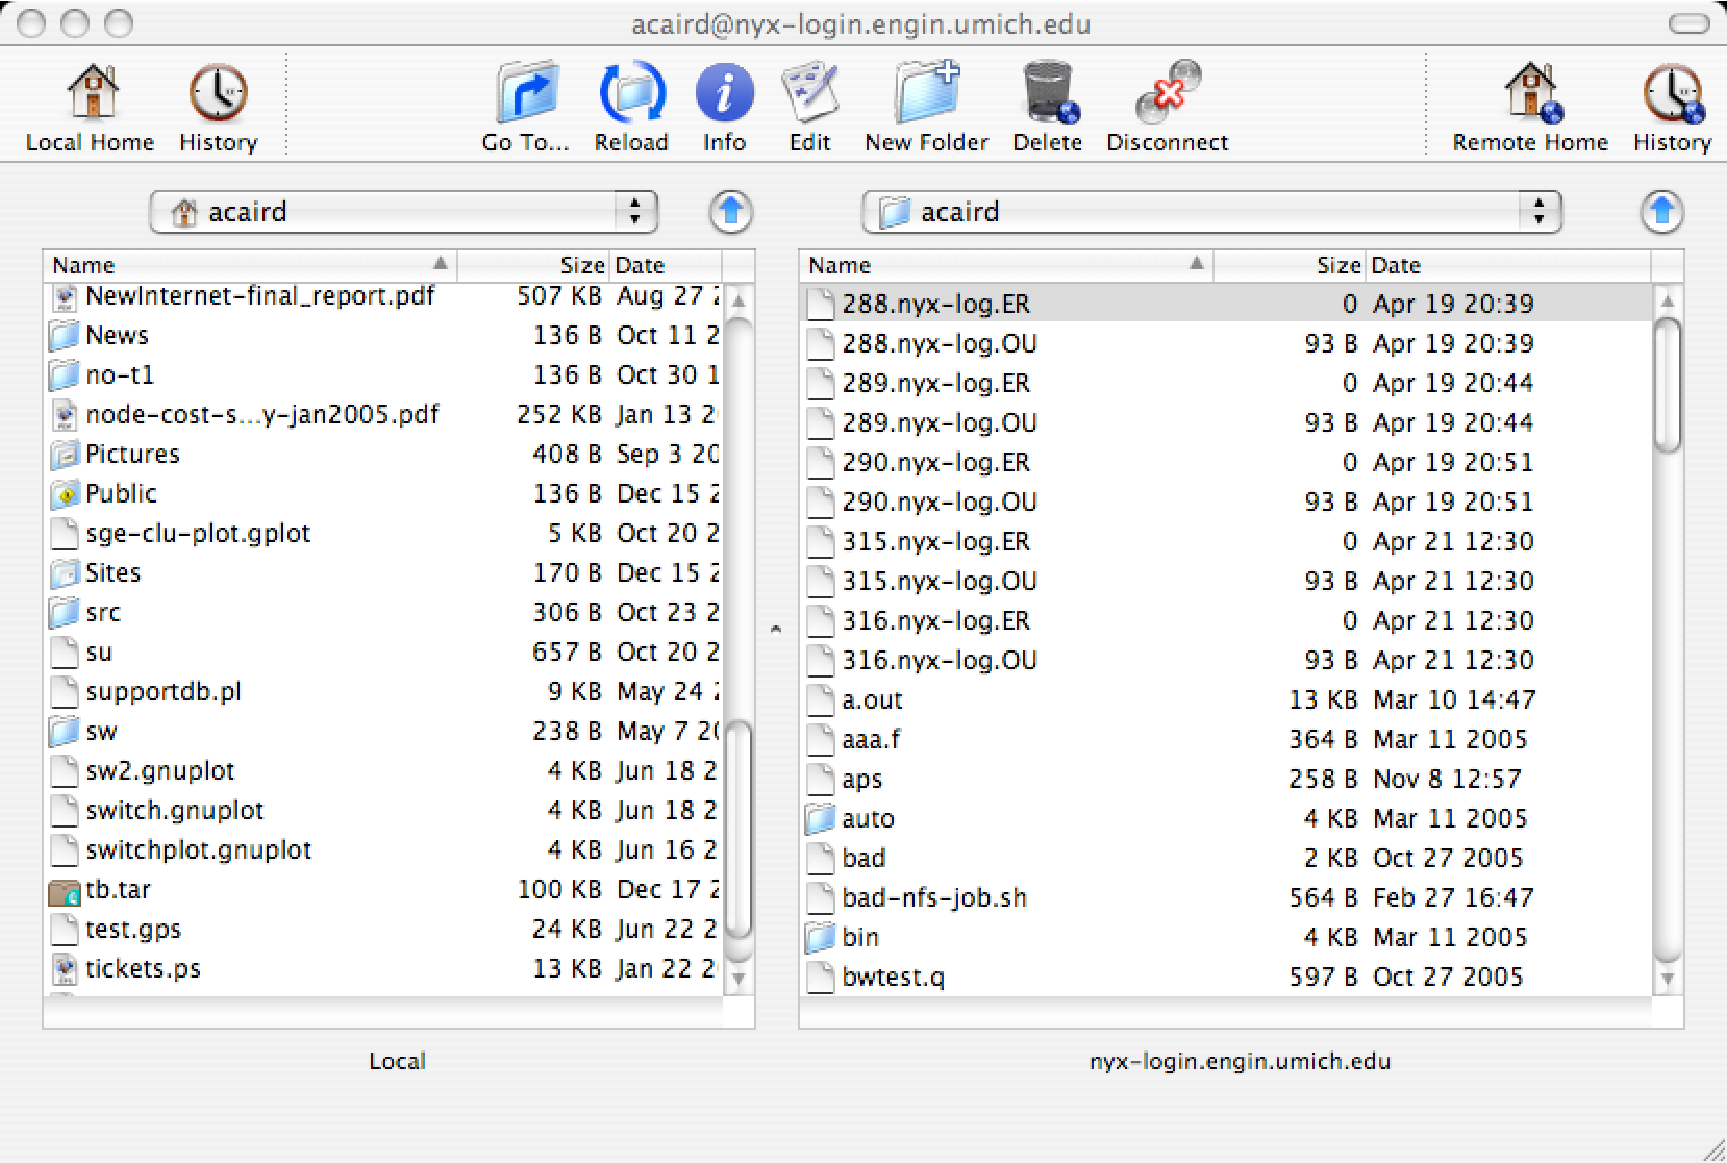
\includegraphics[width=2.5in]{ssh-fugu-connected}\end{center}
    \item You can drag and drop files back and forth
    \end{itemize}
  \end{frame}
  \begin{frame}{File Transfers: Mac}
    \begin{itemize}
    \item There are other programs besides Fugu
    \item Fugu: \url{http://rsug.itd.umich.edu/software/fugu/}
    \item Built-in \texttt{scp}/\texttt{sftp} from Terminal
    \item Rbrowser: \url{http://www.rbrowser.com/}
    \item Fetch: \url{http://fetchsoftworks.com/}
    \item lots of others, see Google
    \end{itemize}
  \end{frame}
\begin{frame}[fragile]
    \frametitle{File Transfers: Linux}
    \begin{itemize}
    \item Using \texttt{scp}:\\
      \tiny
\begin{verbatim}
% scp -r src nyx-login:
Password:
[...]
MP_memcpy.c          100% |*******************************************|  6784       00:00
armci.c              100% |*******************************************|  7590       00:00
gm.c                 100% |*******************************************|  6432       00:00
gpshmem.c            100% |*******************************************|  2611       00:00
ib.c                 100% |*******************************************| 31924       00:00
[...]
\end{verbatim}
      \normalsize
    \item Using \texttt{sftp}:\\
      \tiny
\begin{verbatim}
% sftp nyx-login
Connecting to nyx-login...
Password: 
sftp> 
\end{verbatim}
      \normalsize
    \item This works from the Mac Terminal, too.
    \end{itemize}
\end{frame}
  \subsection{Logging into the clusters}
  \begin{frame}{Logging in}
    \begin{itemize}
      \item<1-> Your login is your Uniquname
      \item<1-> Your password is your ITD/ITCS Kerberos password (Level 1 password)
      \item<1-> Use \texttt{ssh} to connect to the clusters
      \item<2-> All access is command line --- there is no graphical access to the clusters; any 
	graphical pre- or post-processing should be done on your own computer
      \item<3-> For tutorials on using Linux, see:
	\begin{itemize}
	  \item
\href{http://www.engin.umich.edu/caen/technotes/introunix/}{Introduction to Linux}\\
             \tiny\url{http://www.engin.umich.edu/caen/technotes/introunix/}\normalsize
          \item \href{http://www.engin.umich.edu/caen/technotes/advancedunix/}{Advanced Linux}\\
             \tiny\url{http://www.engin.umich.edu/caen/technotes/advancedunix/}\normalsize
          \item \href{http://www.engin.umich.edu/caen/technotes/unixcommands/}{Linux Commands}\\
             \tiny\url{http://www.engin.umich.edu/caen/technotes/unixcommands/}\normalsize
	\end{itemize}
    \end{itemize}
  \end{frame}
  \begin{frame}{Logging in: Windows}
    \begin{itemize}
    \item Putty is a freely available SSH client for windows\\
      \url{http://www.chiark.greenend.org.uk/~sgtatham/putty/}
    \item To log in, enter the host as shown:
      \begin{center}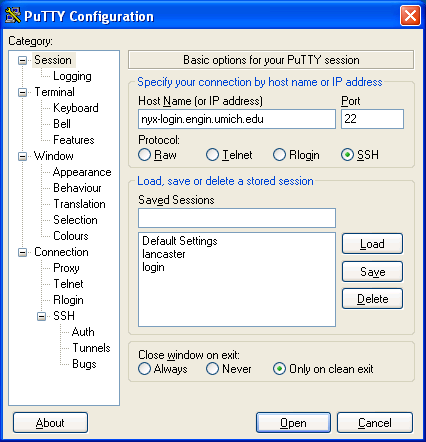
\includegraphics[height=2.25in]{ssh-putty-login}\end{center}
    \end{itemize}
  \end{frame}
  \begin{frame}{Logging in: Windows}
    \begin{itemize}
    \item Then enter your Uniqname and password and you'll get the shell prompt:
      \begin{center}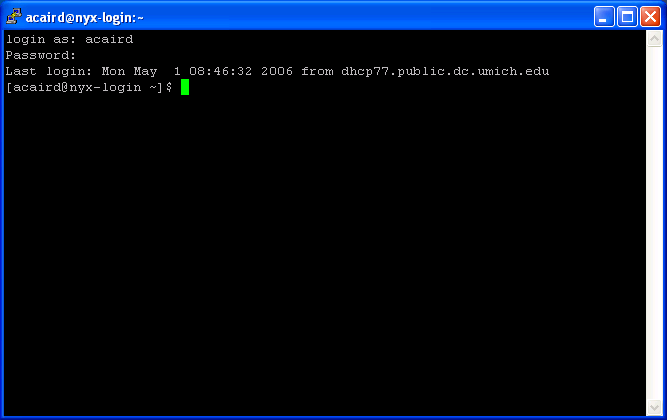
\includegraphics[height=2.4in]{ssh-putty-terminal}\end{center}
    \end{itemize}
  \end{frame}
  \begin{frame}{Logging in: Mac}
    \begin{itemize}
    \item Use the included SSH client from the Terminal program: \\
      \begin{center}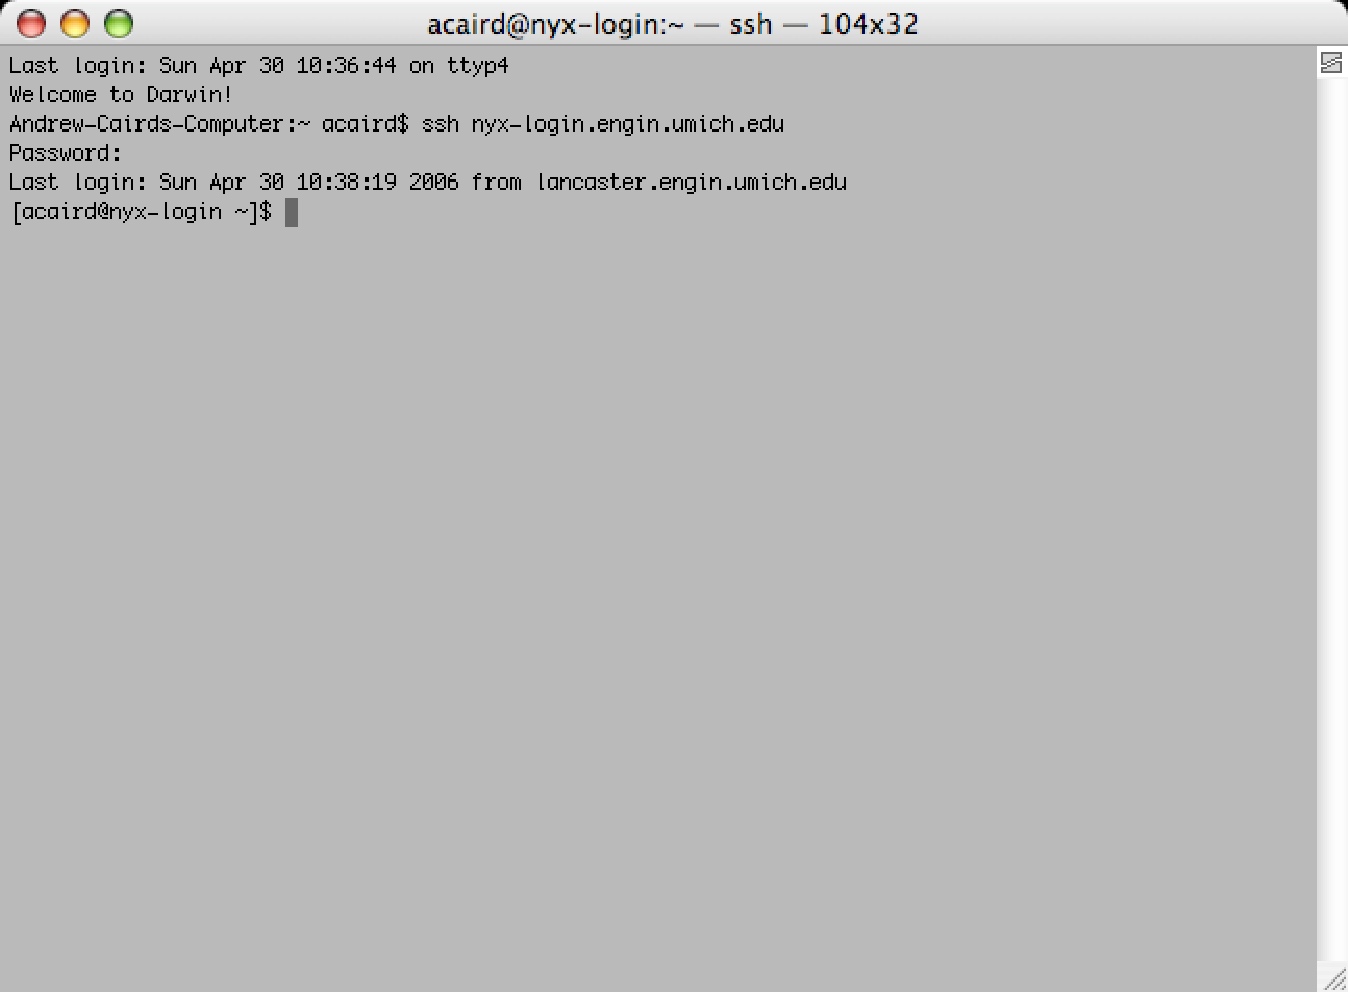
\includegraphics[height=2.8in]{ssh-terminal}\end{center}
    \end{itemize}
  \end{frame}
  \begin{frame}{Logging in: Linux}
    \begin{itemize}
    \item Use the included SSH client from and shell: \\
      %\includegraphics[height=2.8in]{ssh-shell}
    \end{itemize}
  \end{frame}
  \section{Mechanics: Usage}
  \subsection{Compiling programs}
  \begin{frame}{Tools}
   \begin{block}{Tools}
    \begin{itemize}
    \item<1- > All of the standard GNU/Linux tools are also available: \texttt{make},
      \texttt{autoconf}, \texttt{awk}, \texttt{sed}, \texttt{Perl}, \texttt{Python},
    \item<2- > We support \texttt{emacs}, \texttt{vi\{m\}}, and \texttt{nano} (a 
      \texttt{pico}-like editor) on the clusters.
      etc.
    \item<3-| alert@1-> Only use \texttt{notepad} on Windows!
    \item<3-| alert@1-> If made on windows fix with \texttt{dos2unix filename}
    \end{itemize}
   \end{block}
  \end{frame}
  \subsection{The Batch System}
  \begin{frame}{Introduction to the PBS Batch System}
    \begin{itemize}
    \item All access to the compute nodes (everything other than the login node)
      is via the batch system
    \item We use a system called Torque, it is derived from PBS
    \item The batch system controls access to queues
    \item The scheduling system decides if and where jobs can run
    \item<2-> There is one general queue \texttt{cac}
    \item<2-> There are many private queues for people who own or rent nodes
	%fix this
    \item<2-> If you don't know use the \texttt{route} queue
    \end{itemize}
  \end{frame}
  \begin{frame}{Introduction to the PBS Batch System}
    The steps to using the batch system are:
    \begin{enumerate}
    \item Create a batch file: this is a short (5-15 lines) text file with some
      batch commands and the commands to run your program
    \item Submit the file to the batch system
    \item Check on the status of your job
    \item Delete your job if you want to cancel it
    \end{enumerate}
  \end{frame}
\begin{frame}[fragile]
  \frametitle{Creating a PBS Batch File}
A simple single cpu example
  \begin{semiverbatim}
\uncover<1->{#!/bin/sh}
\uncover<1->{#PBS -N 1-cpu}
\uncover<2->{#PBS -l nodes=1,walltime=1:00:00}
\uncover<3->{#PBS -m abe}
\uncover<3->{#PBS -M brockp@umich.edu}
\uncover<4->{#PBS -q route}
\uncover<5->{#PBS -joe}
\uncover<6->{#PBS -V}
\uncover<7->{cd ~/input1dir/}
\uncover<7->{mcnp5.mpi i=input o=output r=restart}
  \end{semiverbatim}
\end{frame}
\begin{frame}[fragile]
  \frametitle{Creating a PBS Batch File}
A more complicated example:
  \begin{semiverbatim}  
\uncover<1->{#!/bin/sh}
\uncover<1->{#PBS -N mcnp-8x2}
\uncover<2->{#PBS -l nodes=8:ppn=2,walltime=8:00:00}
\uncover<3->{#PBS -q route}
\uncover<4->{#PBS -M brockp@umich.edu}
\uncover<4->{#PBS -m ae}
\uncover<5->{#PBS -j oe}
\uncover<6->{#PBS -V}
\uncover<6->{cd \$\{HOME\}/input2/}
\uncover<7->{echo "I ran on: "}
\uncover<7->{cat \$PBS\_NODEFILE}
\uncover<8->{mpirun -np 16 mcnp5.mpi i=input2 o=output2 r=restart2}
  \end{semiverbatim}  
\end{frame}
\begin{frame}[fragile]
  \frametitle{Submitting, Checking, and Deleting Batch Jobs}
  \begin{itemize}
  \item<1-> After you create your PBS script, you need to submit it:\\
  \tiny
\begin{semiverbatim}
$ qsub  mcnp.q 
542.nyx-login.engin.umich.edu
\end{semiverbatim}
\normalsize
  \item<2-> After you submit your script, you can check on the status of your
job:\\
  \tiny
\begin{semiverbatim}
$ qstat -au brockp
nyx-login.engin.umich.edu: 
Job ID               Username Queue    Jobname    SessID NDS   TSK Memory Time  S Time
-------------------- -------- -------- ---------- ------ ----- --- ------ ----- - -----
542.nyx-login.engin. brockp   short    mcnp-8x2     18922     8  --    --  08:00 R 00:00

$ checkjob 542
[... lots of output ...]
\end{semiverbatim}
\normalsize
  \item<3-> If you want to delete your job:\\
\tiny
\begin{semiverbatim}
$ qdel 542
\end{semiverbatim}\normalsize
  \end{itemize}
\end{frame}
\begin{frame}[fragile]
 \frametitle{PBS Email}
PBS will send an email at the start and end of your job if you use the
\texttt{-m} and \texttt{-M} options in your PBS script.  The email after a job
completes successfully looks like:
\tiny
\begin{verbatim}
Date: Sun, 30 Apr 2006 12:50:17 -0400
From: adm <adm@nyx-login.engin.umich.edu>
To: "Palen, Brock E" <brockp@umich.edu>
Subject: PBS JOB 542.nyx-login.engin.umich.edu
----------------------------------------

PBS Job Id: 542.nyx-login.engin.umich.edu
Job Name:   mcnp-8x2
Execution terminated
Exit_status=0
resources_used.cput=13:17:26
resources_used.mem=1220672kb
resources_used.vmem=11146704kb
resources_used.walltime=00:49:57
\end{verbatim}
\normalsize
\begin{itemize}
  \item<2-> Total Consumed CPU time: 47846 Sec.
  \item<2-> Total Real Time: 2997 Sec.
  \item<3-> 16x Faster than 1 CPU 
\end{itemize}
\end{frame}
\section{The Scheduler}
\subsection{Understanding the Scheduler}
\begin{frame}{Understanding the Scheduler}
The scheduler determines what jobs can run, when the can run, and where.  There
are many factors that go into the scheduler's decision.
  \begin{itemize}
  \item<1-> Limits
    \begin{itemize}
    \item<1-> Maximum number jobs eligible for scheduling: 4
    \item<1-> Maximum number of CPUs in use by one person: depends on queue
    \item<1-> Maximum number of jobs in the queue at one time: no limit
    \end{itemize}
  \item<2-> Priority
    \begin{itemize}
    \item<2-> Who you are: user and group level priorities
    \item<2-> How long you've waited: the longer you wait, the higher your
priority
    \item<2-> Your recent usage (fairshare): People with less usage over the
past month will have a higher priority than those with a lot of usage
    \end{itemize}
  \end{itemize}
\end{frame}
\begin{frame}{Understanding the Scheduler}
  \begin{itemize}
  \item<1-> Reservations
    \begin{itemize}
    \item<1-> Advance reservations: holds nodes for users or groups
    \item<1-> Job reservations: scheduler will reserve nodes for the next
several jobs in each queue
    \end{itemize}
  \item<2-> Backfill
    \begin{itemize}
    \item<2-> If the reservations leave holes in the schedule, they may be
filled by short jobs that otherwise would have waited.\\
	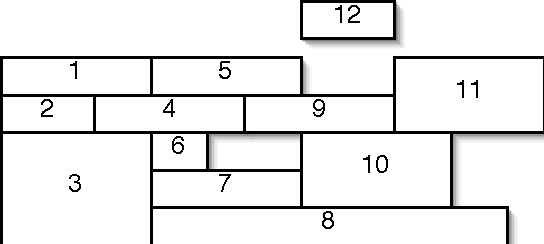
\includegraphics{job-grid}
    \end{itemize}
  \end{itemize}
\end{frame}
\subsection{Scheduler Commands}
\begin{frame}{Understanding the Scheduler}
There are several commands that can give you insight into the scheduler's
decisions.
\begin{itemize}
\item \texttt{showq} --- shows the state of the queue at that moment in time,
showing the running jobs in order of soonest to finish to longest to finish; the
idle jobs in order of priority; and the blocked jobs in the order they were
submitted
\item \texttt{diagnose -p} --- shows the factors that go into computing the
priority for all of the idle jobs
\item \texttt{checkjob \textit{jobnumber}} --- for idle jobs this will show why
the job can't start
\item \texttt{showstart \textit{jobnumber}} --- this makes a (poor) estimate of
when the job will start
\end{itemize}
\end{frame}
\section{Summary}
\subsection{Resources and Access}
\begin{frame}{Summary}
 \begin{itemize}
  \item Resources
   \begin{itemize}
    \item Lots of CPUs
    \item A reasonable amount of software
    \item Watch or subscribe to \url{http://cac.engin.umich.edu} for updates
   \end{itemize}
   \item Access
    \begin{itemize}
     \item All access is via the SSH family of commands: \texttt{ssh},
\texttt{sftp}, \texttt{scp}
     \item There are lots of clients for these commands for the different
platforms
     \item There is no graphical access, everything is via the command line
    \end{itemize}
 \end{itemize}
\end{frame}
\subsection{Job Management}
\begin{frame}{Summary}
 \begin{itemize}
   \item Job Submission
     \begin{itemize}
     \item Every job needs a PBS script file
     \item Two most important commands: \texttt{qsub} and \texttt{qstat -au \textit{uniqname}}
     \end{itemize}
   \item Job Scheduling
     \begin{itemize}
     \item Scheduling depends on a lot of factors, it is best to submit jobs and let the
scheduler optimize for their start.
     \end{itemize}
 \end{itemize}
\end{frame}
\subsection{Contact}
\begin{frame}{Summary}
 \begin{itemize}
 \item News: \url{http://cac.engin.umich.edu}
   \begin{itemize}
    \item RSS feed
    \item New of changes, outages, other pertinent piece of information
   \end{itemize}
  \item Contact: \url{cac-support@umich.edu}
   \begin{itemize}
    \item Questions or concerns should be sent here (not to an individual) since
this is read by six people.  The odds of a quick reply are best this way.
    \item We aren't parallel programmers, but we'll do what we can to help.
   \end{itemize}
 \end{itemize}
\end{frame}
\begin{frame}{Example}
 \begin{example}
  Open a shell....
  \begin{enumerate}
   \item<1>  \texttt{cp -r \textasciitilde brockp/mcnp\_example ~/}
   \item<2>  \texttt{cat mcnp.q}
   \item<3>  \texttt{module load mcnp5}
   \item<4>  \texttt{qsub mcnp.q}
   \item<5>  \texttt{qstat -u \$USER}
  \end{enumerate}
 \end{example}
\end{frame}
\end{document}
